\documentclass{article}\usepackage[]{graphicx}\usepackage[]{color}
%% maxwidth is the original width if it is less than linewidth
%% otherwise use linewidth (to make sure the graphics do not exceed the margin)
\makeatletter
\def\maxwidth{ %
  \ifdim\Gin@nat@width>\linewidth
    \linewidth
  \else
    \Gin@nat@width
  \fi
}
\makeatother

\definecolor{fgcolor}{rgb}{0.345, 0.345, 0.345}
\newcommand{\hlnum}[1]{\textcolor[rgb]{0.686,0.059,0.569}{#1}}%
\newcommand{\hlstr}[1]{\textcolor[rgb]{0.192,0.494,0.8}{#1}}%
\newcommand{\hlcom}[1]{\textcolor[rgb]{0.678,0.584,0.686}{\textit{#1}}}%
\newcommand{\hlopt}[1]{\textcolor[rgb]{0,0,0}{#1}}%
\newcommand{\hlstd}[1]{\textcolor[rgb]{0.345,0.345,0.345}{#1}}%
\newcommand{\hlkwa}[1]{\textcolor[rgb]{0.161,0.373,0.58}{\textbf{#1}}}%
\newcommand{\hlkwb}[1]{\textcolor[rgb]{0.69,0.353,0.396}{#1}}%
\newcommand{\hlkwc}[1]{\textcolor[rgb]{0.333,0.667,0.333}{#1}}%
\newcommand{\hlkwd}[1]{\textcolor[rgb]{0.737,0.353,0.396}{\textbf{#1}}}%

\usepackage{framed}
\makeatletter
\newenvironment{kframe}{%
 \def\at@end@of@kframe{}%
 \ifinner\ifhmode%
  \def\at@end@of@kframe{\end{minipage}}%
  \begin{minipage}{\columnwidth}%
 \fi\fi%
 \def\FrameCommand##1{\hskip\@totalleftmargin \hskip-\fboxsep
 \colorbox{shadecolor}{##1}\hskip-\fboxsep
     % There is no \\@totalrightmargin, so:
     \hskip-\linewidth \hskip-\@totalleftmargin \hskip\columnwidth}%
 \MakeFramed {\advance\hsize-\width
   \@totalleftmargin\z@ \linewidth\hsize
   \@setminipage}}%
 {\par\unskip\endMakeFramed%
 \at@end@of@kframe}
\makeatother

\definecolor{shadecolor}{rgb}{.97, .97, .97}
\definecolor{messagecolor}{rgb}{0, 0, 0}
\definecolor{warningcolor}{rgb}{1, 0, 1}
\definecolor{errorcolor}{rgb}{1, 0, 0}
\newenvironment{knitrout}{}{} % an empty environment to be redefined in TeX

\usepackage{alltt}
\usepackage{hyperref}
\usepackage{amsmath}
\IfFileExists{upquote.sty}{\usepackage{upquote}}{}
\begin{document}

\title{Logistic Growth of a Population App}
\author{Jacob S. Townson}
\date{April 5, 2016}
\maketitle



\begin{abstract}

The classroom is becoming more of a technological advanced place with each passing year. It is becoming increasingly more common to use apps and other electronic forms of learning to be present in a class. In order to try to see this in action, our group has made an app for an Evolution and Ecology course at our college. This app was made using different probability models and theoretical differential equations in a Shiny App made in R Studio. The app is used to show/simulate a population's growth when there is a specific carrying capacity, birth rate, and death rate. The app's purpose is to help teach the biology class this lesson of a population with a carrying capacity through the use of dynamic graphs and an interesting yet easy to use interface. The app has been successful in the implementation behind it, as it is fully functional and ready for the classroom. To test it's use in a class, we have given a survey to two separate classes to test their knowledge of the subject. One class used the app and the other did not. *Insert results here*

\end{abstract}

\pagebreak

\tableofcontents

\pagebreak

\section{Introduction}

\subsection{Question}

Over the summer of 2015, I worked in a research group on Georgetown College's campus with Dr. Homer White and fellow student Andrew Giles. Originally, we were working on learning about Data Science, and began taking classes in a Data Science Specialization Course online. After Andrew and I learned some of the material, Dr. White recommended we work on Shiny apps, and make a successful Shiny app by the end of the summer. We were approached by a biology professor, Dr. Timothy Griffith, with a project to make a shiny app for his Evolution and Ecology class at Georgetown. We chose to do this project and made a functional and easy to use app for the class. So the question arose, how well will this app work in the classroom setting with biology students? In other words, does using an app rather than learning the full and heavy math behind the model help students more, or does it mask too much of the details?

As mentioned, our app works with the math behind an evolution and ecology course. The app is used to show/simulate a population's growth when there is a specific carrying capacity, birth rate, and death rate. Below I will explain the design and methods we used to make the app. To see our code, and more details on how we did our work, feel free to visit our GitHub repository for this project at \url{https://github.com/obewanjacobi/shinyBio/tree/master}. Or to see the app itself, visit \url{https://obewanjacobi.shinyapps.io/logistic}.

\subsection{Significance}

Using technology in the classroom has been an up and coming subject in the past few years. Schools all around the US and even out of the country have begun bringing in new tech to try and help enhance the learning experience to make it easier for students. So, the reason that my question matters is because if apps like these are easy to make, if they are helpful, then we can start integrating them into classes more regularly. Students wouldn't be required to try and understand the gory details of a subject that don't apply to them, unless they really want to. The teacher can easily regulate what is shown at one certain time versus another. When asked, future teachers prefer having apps because it helps to get all of the students involved in the learning process, as well as organize thoughts to help manage the class and how they learn.

Studies show especially for the subject of evolution and ecology (the course that this app was made for), because understanding the theory behind many things requires the conceptualization of some fairly difficult mathematics, biology students have difficulty learning it. This is referenced in the article \textit{Creative Education} (2011) when they say "...population dynamics is a complex branch of population ecology that has an essentially quantitative nature. The effective assimilation of this topic should consider basic aspects of population theory, which involves the conceptual understanding of mathematical models." People are looking for new ways to teach this subject, and many others as well. Using an app like this one could make a huge difference to students everywhere. Other studies, like Scott McDaniel's article in \textit{EScholarship}, show that the entrance of apps and applets into the classroom have actually increased results on tests. So making these apps more integrated into the way we teach could actually help students learn more easily.

\subsection{Population Biology Overview}

Population biology is a branch of biology involving evolution, ecology, and behavioral biology. It is also heavily reliant on some knowledge of mathematical modelling. Unfortunately being on the more mathematical sides of things, it is difficult for myself to define population biology in such a way that I convey it correctly. Luckily, Don Alstad (an actual biologist) puts it quite well in his book \textit{Basic Populus Models of Ecology} by describing: "Population biology is a quantitative science dealing with changes in the size and composition of populations, and population biologists often use mathematical models to infer population dynamics." Because students aren't necessarily population biologists yet, this is where my app development group comes into play to help with the education of these students so that they can see the importance of mathematical modelling in population biology.




\section{Methods}



\subsection{Tools}

Before going into the design and models used in the app, one must first understand what R and RStudio are. R is a coding language and environment, mostly used for statistical purposes. I won't go into the entire history of how the language was made, but it is based on of the S language. When I say that it's a language and environment, I mean that it is a language in that R is a type of coding language, and it's an environment because it is a system of tools rather than a group of seemingly unrelated tools as is the case with some other languages. It has a large range of graphical, and many different kinds of statistical abilities, thus why it is extremely useful for this project.

RStudio is the IDE, or integrated development environment for R. What that means is that RStudio can be used to make R code and run it, while also helping along the way by attempting to help correct errors when they are made. This is where our group did all of our coding with R to make the app. 

The other tools that were essential to our project were git and GitHub. Git is a version control system, which means that it is a method used for keeping track of the versions made of software. We used git to handle when we would make changes to our app overtime. Having version control is important so that if something went wrong, we could trace it back to a certain version that we had made. 

GitHub is used for similar things, however it has a nicer user interface, and is on the internet for everyone to see. So when we would make an updated version of the app and commit it using git, we would then "push" our changes to GitHub so that the rest of the group could get the newest version of the app. This helped so that the entire group was on the same page of where the app was in development. If you would like to see the GitHub repository with all of our work, please visit \url{https://github.com/obewanjacobi/shinyBio/tree/master}. Feel free to make an account as well, that way you can comment on any of our work by using the "Issues" button on GitHub. This helps us so that we can make any necessary changes as soon as possible.






\subsection{Mathematical Modeling}

Before one can understand the methods and reasoning behind each step of making this app, one must first understand where the math comes from that the app is based on. Our model relies on the use of differential equations and their solutions for the theoretical portion of the app, and probability and statistical models for the simulations made and run in the app. One last thing to understand before I delve into how we made the models used in the app is the notation and variables that we used for the models themselves. Let us establish the following notation:

\begin{itemize}
\item \(n_0 =\) initial population

\item \(n(t) =\) population at time \(t\), sometimes abbreviated as \(n\)

\item \(b =\) unconstrained birth rate (or the maximum birth rate)

\item \(d =\) unconstrained death rate (or the minimum death rate)

\item \(m =\) carrying capacity (max population that an environment can safely sustain)

\item \(b_t =\) per capita birthrate at time \(t\)

\item \(d_t =\) per capita number of deaths at time \(t\)
\end{itemize}

\subsubsection{Differential Equations}

This section will explain how we found the differential equation that was used in the theoretical calculation of the population and its growth. We will begin with what we know, and expand from there using our previous definitions given.

We know that the rate of population growth is going to be the the number of rabbits times the birth rate at that specific time minus the per capita number of deaths at that specific time. To put this in terms of math, we would write it as \(\frac{dn}{dt} = nb_t-d_t\) which simplifies to be 

\begin{equation}
\frac{dn}{dt} = n\left(\frac{b-d}{m}\right)(m-n) 
\end{equation}

\noindent by our model when \(b > d\). We will look at the case when \(d > b\) at the end of this section. To solve this theoretical equation, we must use knowledge of differential equations. From here we will split into 3 cases, when \(n_0 =m\), \(n_0 > m\), and \(n_0 < m\). 

To start, take note of the almost trivial answer when \(n_0 = m\). Here, I propose that based off of our differential equation we made, we can find that \(\frac{dn}{dt} = 0\). While proving this using differential equations and algebra is difficult and hard to follow mathematically, let's look at it from a logical point of view. If a population starts off at it's carrying capacity, it would only make sense that it would not grow anymore or drop any lower than that value. If we solve the differential equation using the initial value of \(n_0 = m\), we find that the equation simplifies in such a way that in fact for any time value, \(n=m\). This tells us that the theoretical equation is a constant, which makes sense considering that if a population starts off at it's carrying capacity, theoretically it wouldn't grow (even though this isn't necessarily true, which we make note of with our simulation).

Next, we must look at our other two cases, \(n_0 > m\) and \(n_0 < m\). For each we want to move all of the \(n\) values to one side of the equation to make it easy to integrate. This leads us to get 

\begin{equation}
\int \frac{dn}{n(m-n)} = \int \frac{b-d}{m} dt = \frac{b-d}{m} t + C
\end{equation}

\noindent where C is some constant that we will find later. So now we want to integrate the left side of the equation. In order to do this, we will need to use partial fractions to simplify it to make it easy to integrate. After doing this, we get that 

\begin{equation}
\int\left(\frac{1}{mn}+\frac{1}{m^2-mn}\right)dn = \frac{b-d}{m} t + C
\end{equation}

\noindent When we integrate this simpler integral and apply some natural log rules, we get that 

\begin{equation}
\frac{1}{m}\left(\ln\left|\frac{n}{m-n}\right|\right) = \frac{b-d}{m} t + C
\end{equation}

\noindent Note the absolute value in the above equation. This is why we need two cases for this one integral. For the case of \(m > n_0\), the value inside the absolute value is unchanged. From here, we want to find what the \(C\) value is. In order to do this, let \(t=0\) so \(n=n_0\). After solving equation (4) for \(C\), we get that \(C = \frac{1}{m}(ln(\frac{n_0}{m-n_0}))\). This gives us that 

\begin{equation}
\frac{1}{m} \ln\left(\frac{n}{m-n}\right) = \frac{b-d}{m}t + \frac{1}{m}\ln\left(\frac{n_0}{m-n_0}\right)
\end{equation}

\noindent Now we can simply solve the equation for \(n\). This mostly just involves some elementary algebra, which leads us to get that 

\begin{equation}
n = \frac{m}{1+\left(\frac{m-n_0}{n_0}\right)\mathrm{e}^{(d-b)t}}
\end{equation}

\noindent if \(m > n_0\). This is our standard equation for the theoretical model. However as mentioned, we must realize that you cannot take the natural log of a negative number hence our third case of \(n_0 >m\). To account for this we must go back to equation (4). Here, we notice that because \(n_0 > m\) we get a negative value inside the natural log giving us the new equation:

\begin{equation}
\frac{1}{m}\left(\ln\left(\frac{n}{n-m}\right)\right) = \frac{b-d}{m} t + C
\end{equation}

\noindent Here we have taken the absolute value of the number inside the natural log. Next we can go through the steps as we did in the second case. After doing these algebra steps, we find that 

\begin{equation}
n= \frac{-m}{\frac{n_0-m}{n_0}\mathrm{e}^{(d-b)t}-1}
\end{equation}

\noindent if \(n_0 > m\). This is our model for the theoretical graph when \(b > d\).
\bigskip

\begin{figure}
\begin{knitrout}
\definecolor{shadecolor}{rgb}{0.969, 0.969, 0.969}\color{fgcolor}

{\centering 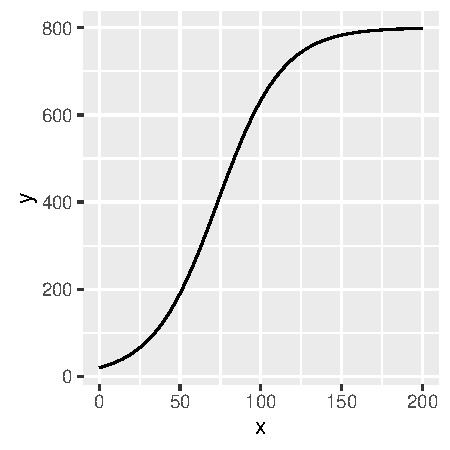
\includegraphics[width=\maxwidth]{figure/unnamed-chunk-2-1} 

}



\end{knitrout}
\caption{This graph is an example plot of what the population of rabbits would look like if \(b > d\) and \(m > n_0\). Here \(n_0 = 20\), \(m = 800\), \(b = .1\), and \(d = .05\).}
\end{figure}

\begin{figure}
\begin{knitrout}
\definecolor{shadecolor}{rgb}{0.969, 0.969, 0.969}\color{fgcolor}

{\centering 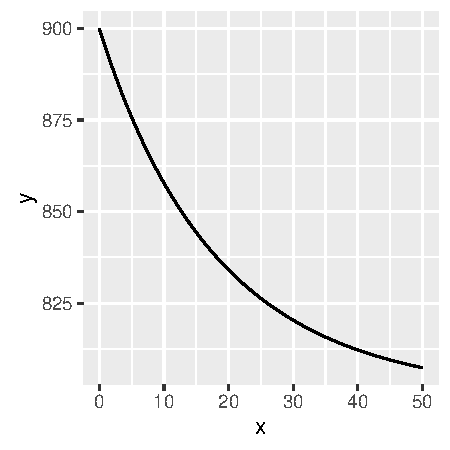
\includegraphics[width=\maxwidth]{figure/unnamed-chunk-3-1} 

}



\end{knitrout}
\caption{This graph is an example plot of what the population of rabbits would look like if \(b > d\) and \(m < n_0\). Here \(n_0 = 900\), \(m = 800\), \(b = .1\), and \(d = .05\).}
\end{figure}

In order to be sure of our deterministic model, we wanted to consult a biology text to see if there was anything similar done before. After some research, our group found that this model follows the theoretical equation for other biologists as well. Their equation was 

\begin{equation}
N(t) = \frac{K}{1+(\frac{K-N(0)}{N(0)})\mathrm{e}^{-rt}}
\end{equation}

\noindent found by Roughgarden(1979), Emlen(1984), and Neuhauser(2000). This relates to our equation because \(N(t) = n\), \(K=m\), \(N(0)=n_0\), and \(r = b-d\). In order to see example graphs of this deterministic model, consult Figures 1 and 2.

\begin{figure}
\begin{knitrout}
\definecolor{shadecolor}{rgb}{0.969, 0.969, 0.969}\color{fgcolor}

{\centering 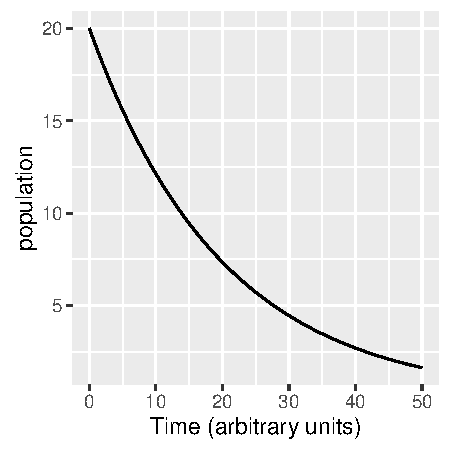
\includegraphics[width=\maxwidth]{figure/unnamed-chunk-4-1} 

}



\end{knitrout}
\caption{This graph is an example plot of what the population of rabbits would look like if \(d > b\). Here \(n_0 = 20\), \(b = .05\), and \(d = .1\).}
\end{figure}

Now let's look at the case of when \(d > b\). This case is unusual compared to our work above because here, the carrying capacity is insignificant. To explain why, imagine a population of rabbits whose death rate is higher than their birth rate. In other words, the rabbits are dying faster than they can be born. If this is the case, then what does a carrying capacity even matter? The rabbits will most likely die off either way, no matter what the population can or won't support. So for this part of the model, we don't consider the value of \(m\) as it doesn't affect the situation. Instead, we will write the differential equation as 

\begin{equation}
\frac{dn}{dt} = n(b-d)
\end {equation}

\noindent After some simple integration and solving the equation for \(n\), we see that the equation for \(n\) in this situation gives us that 

\begin{equation}
n = n_0 \times \mathrm{e}^{(b-d)t}
\end{equation}

Looking at the example graph of equation (11) in Figure 3 where \(d > b\) shows us that theoretically this graph would make sense. The population starts at the initial population then decreases based on how much greater the unconstrained death rate is compared to the unconstrained birth rate. Thus we have our complete deterministic model for the population based on multiple cases. 

\subsubsection{Probability Model}

In order to run simulations to convey to the students that the deterministic model isn't always true, we need a probability model for the simulation to follow. This is where the variables defined before as being reliant on time come into play. They are reliant on time is because at each given time interval, the app will run a simulation based on what the previous time values were. We will get more into the programming of this later, but for now, here is the math behind our model.

To begin, let's define some variables that will be needed to create our model:

\begin{itemize}
\item \(L_t =\) number of litters at time \(t\)

\item \(S_t^i =\) size of the \(i^{th}\) litter born at time \(t\). These are independent of each other and of \(L_t\)

\item \(B_t =\) number of births at time \(t\)
\end{itemize}

\noindent These are random variables that are dependent on time. Random variables are variables that are dependent on chance factors. To put this in perspective of the app, the number of baby rabbits born to a litter won't always be the same. Rather, the number of babies is dependent on multiple chance factors such as health of the rabbits, rabbit genetics, etc. To represent this chance variation, we will use a Poisson distribution to describe the variables here and give us our simulated data. A Poisson distribution is convenient for this situation because it is used to express the probability of a given number of events happening in a certain interval of time. So for us, this is used to represent the number of rabbits born to a litter at time \(t\), and the number of litters born at time \(t\). 

First, one must understand the concept of an expected value. An expected value is an average value of a variable that you would expect to happen if you gathered an infinite amount of data for the subject, and is found in different ways depending on the distribution used to describe that variable. In our case, we are using a Poisson distribution to describe the population of rabbits. Luckily, RStudio can calculate this easily for us. For now, we will simply represent the expected value of a random variable as \(E(X)\) where \(X\) is the random variable. 

A Poisson distribution is useful to our purposes because of the shape of the distribution. To show an example of this, view Figure 4. Here, the \(y\) axis represents the probability of \(x\) happening, and the \(x\) axis represents the number of occurrences of the event that \(x\) defines. Notice that the values seem to peak somewhere around 8, because in Figure 2, the expected value (or \(\lambda\) for this kind of distribution) is 8. The graph then has a tail (decrease towards 0) as the number of occurrences approaches infinity. This shape fits our situation of rabbit births quite well, as we know there will be an expected value of rabbit births, but we also know that the chance variation for rabbit births is likely to trail off to large numbers as well, but this is much less likely to happen. 

\begin{figure}
\begin{knitrout}
\definecolor{shadecolor}{rgb}{0.969, 0.969, 0.969}\color{fgcolor}

{\centering 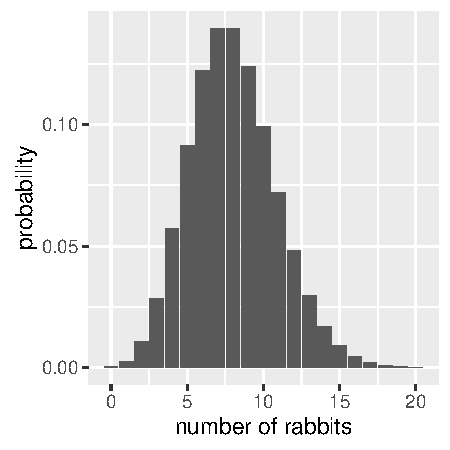
\includegraphics[width=\maxwidth]{figure/unnamed-chunk-5-1} 

}



\end{knitrout}
\caption{This histogram represents a standard Poisson distribution with an expected value of 8.}
\end{figure}

Now we can proceed with the explanation of the model, so let's make two more variables just to help set up the overall calculations: let 

\begin{equation}
s_t = E(S_t^i)$$ and $$l_t = \frac{E(L_t)}{n}
\end{equation}

\noindent where \(s_t\) is the expected litter size and \(l_t\) is the per capita number of litters to expect in the population. We know that the number of births at time \(t\) will be the sum of the sizes of all of the litters, so 

\begin{equation}
B_t = \sum_{i=1}^{L_t} S_t^i 
\end{equation}

We call the per capita birth rate \(b_t = \frac{E(B_t)}{n}\), as we defined before. We would like to show then that the expected number of births is the expected number of litters times the expected size of the litters, or \(E(B_t) = E(S_t^i)\times E(L_t)\). To do this, we must use properties of expected values. First take the expected value of \(B_t\), giving us 

\begin{equation}
E(B_t) = E\left(\sum_{i=1}^{L_t} S_t^i\right)
\end{equation}

\noindent From this using conditional expected value properties we see that 

\begin{equation}
\begin{split}
E(B_t) & = E(E(B_t | L_t)) \\
& = E\left(E\left(\sum_{i=1}^{L_t} S_t^i | L_t\right)\right)
\end{split}
\end{equation}

\noindent In words, equation (13) means we want the expected value of the expected value of the sum given \(L_t\). We can assume that \(S_t\) is independent of \(L_t\) here because the litter sizes do not depend on the number of litters birthed in a population. To explain a real life situation, to say that these things are dependent is equivalent to saying that if a rabbit is near or witnesses another rabbit having babies, it will control or naturally have a different amount of births because of this, which isn't true. Thus we can make our assumption. Now using properties of expected values and independent conditional circumstances, we then simplify such that \(E(B_t) = E(\sum_{i=1}^{L_t} s_t)\). The sum can now be changed such that \(E(B_t) = E(L_t \times s_t)\), and because \(s_t\) is a constant here, we know that 

\begin{equation}
E(B_t) = s_t \times E(L_t)
\end{equation}

\noindent When (14) is simplified based on our definitions we can write it as

\begin{equation}
b_t = s_t\times l_t
\end{equation}

\noindent Which completes our proof. 

 The \(s_t\) and the \(l_t\) are what we simulate using the \textit{rpois()} function in R, which as previously stated, we will address more later. Our group needed an expected average litter size, so we simply googled the average rabbit litter sizes for this value. The number born to each litter isn't entirely important to our model because the model still accounts for carrying capacity and theoretical growth rather than the litters affecting the outcome. We found that the average litter sizes for rabbits was \(8\), so we let the 

\begin{equation}
s_t = \frac{8\sqrt{b_t}}{\sqrt{b}}
\end{equation}

and 

\begin{equation}
l_t = \frac{\sqrt{b_t}}{8}\times \sqrt{b}
\end{equation}

\noindent in order to be able to calculate the the simulated number of births at time \(t\) based on litter size and number of litters. Using what we have found here, we can associate each litter with a simulated litter size which we will use in two sections of the app, The Field and The Graveyard. These two sections of the app will be addressed when discussing the user interface. It should also be noted that defining \(s_t\) and \(l_t\) is only one way of doing it. We could have made other choices, but we chose these because of how we found the average litter size to be 8 for a standard population of rabbits. This makes the overarching probability model that we will use for the simulation of our app. The final mathematical step is to relate the differential equation to the probability model itself, and using what we find, we can then use that in our code for what we want to accomplish. 









\subsubsection{Checking the Model}

In this section, in order to check the model, we must show that the deterministic and probability models connect. To do this, we have to use everything we have proven, defined, and assumed up to this point in both the deterministic and the probability models. This part is also crucial to the coding of our app because of how the code write up will look. Connecting the two models together helps to make the code writing much more organized and fluid so that the computer won't have to process two ideas at once, making the app run as quickly as possible for the students. 

To begin, let's define one last variable: \(b* = b + \frac{d-b}{2} \left( \frac{n}{m}\right)\). Now, we will be looking at the case of \(b > d\). Let 

\begin{equation}
b_t = max(0, b*)$$ and $$d_t = d + \frac{b-d}{2} \left(\frac{n}{m}\right) + max(0, -b*)
\end{equation}

\noindent Recall that we defined \(\frac{dn}{dt} = nb_t-d_t\) and \(\frac{\frac{dn}{dt}}{n} = (b-d)\left(1-\frac{n}{m}\right)\). Our goal here is to prove that based on what we have found in the deterministic and probability model that 

\begin{equation}
nb_t-d_t = \left(\frac{b-d}{m}\right)(m-n)
\end{equation}

Consider the case where \(b* < 0\) (the case where b* > 0 is similar). Here

\begin{equation}
\begin{split}
nb_t - d_t & = 0 - d - \frac{b-d}{2} \left(\frac{n}{m}\right)- -b* \\ 
& = -d-\frac{b-d}{2} \left(\frac{n}{m}\right) +b + \frac{d-b}{2} \left(\frac{n}{m}\right) \\
& = b-d-(b-d)\left(\frac{n}{m}\right) \\
& =(b-d)\left(1-\frac{n}{m}\right)
\end{split}
\end{equation}

\noindent Thus we have proven that when \(b* < 0\) that our model works. It not only makes sense mathematically, but also through example. Consider the rabbits, it makes sense that the population will grow based off of \((b-d)\) (the unconstrained birth rate minus the unconstrained death rate), but the growth rate will slow as the population \(n\) approaches the carrying capacity \(m\), which is handled by the fraction \(\frac{n}{m}\). 

There is also the case of when \(d>b\). This case is interesting because as we explained before in the Differential Equation section, carrying capacity is not relevant here. Thus, to keep things simple, we just use the unconstrained birth rate and unconstrained death rate to define the birth rate over time and per capita number of deaths over time. In mathematical terms, in this case we simply let \(b_t = b\) and \(d_t=d\). Thus we have covered all of the cases we must check to make sure that our model is correct. 

This concludes the Mathematical Modelling section. Now that we have an accurate model that works correctly, we can move on to the making of the app itself. 










\subsection{App Design - The User Interface}

Before going deep into the app design on the user interface (or UI for short), I invite the reader to experience the app for themselves so that the design process makes more sense. The app can be found at \url{https://obewanjacobi.shinyapps.io/logistic}. 

\subsubsection{Sidebar}

This section of the app is where the students input their values for the graphs and simulations. It is always on the left side of the app, and is dynamic such that when the user changes any input on a slider, the graph will change depending on what they have chosen. The only case where this isn't true is if the user has hit the simulate button, in which case the sidebar simplifies accordingly. The descriptions of the input are described below.

\begin{itemize}

\item \textbf{Time}: This lets you choose the time value displayed on the x axis of the graph under the \textit{Population Size} tab.

\item \textbf{Initial Population}: This lets you choose the initial population, or the y intercept under the \textit{Population Size} tab.

\item \textbf{Birth Rate}: This lets you choose the maximum birth rate for the population. The effective birth rate will change according to how close the population gets to the carrying capacity.

\item \textbf{Death Rate}: This lets you choose the minimum death rate for the population. The effective death rate will change according to how close the population gets to the carrying capacity.

\item \textbf{Carrying Capacity}: This lets you choose the carrying capacity for a population. It could be thought of as the amount of resources a population has to survive/thrive. Note, carrying capacity option is removed if death rate is above birth rate because a carrying capacity doesn't affect this given situation.

\item \textbf{Setting the Seed}: This check box gives the user the option to set the seed of the simulated values. By setting the seed, the user can get the same outcomes for every time the \textit{Simulate} button is pushed while the seed is set to that specific value. When the box is unchecked, the option goes away and the simulation is random again.

\item \textbf{Simulate}: This button runs the app with a new simulation with the given input parameters.

\end{itemize}

\subsubsection{Population Graphs}

This section is the main portion of the application. This is the only tab available before the \textbf{Simulate} button is hit. This tab displays the graphs used to convey information on the population growth. Before the \textbf{Simulate} button is hit, the graph displays only the theoretical results. These theoretical results are what would happen "on average". This means that if we can imagine an infinite amount of populations were observed, the average would look like our theoretical results. If the \textit{Size} button is chosen, then the population size graph will be shown. This graph shows the growth of a population over an arbitrary amount of time as it approaches its carrying capacity. Here the population is conveyed by the red line and the carrying capacity is shown in blue. The next option under this tab is to plot the growth rate. Here the growth rate is plotted against either time or the population itself. This switching between what is plotted on the x axis can help to teach students how the growth rate changes, and makes it more easily understood through a look at it from both perspectives. Similar to this structure, the next option under this tab is to plot the per capita growth rate. Again, the user can choose what to put on the x axis, either time or population to give the user an easier way of understanding depending on their perspective.

The only change that is made under this tab by hitting the \textbf{Simulate} button is that a simulated population is displayed on the \textit{Size} graph. This is conveyed by a black line. This simulated line is made using our model and with the help of the \textit{rpois()} function in R. So this creates a possible outcome for a single population to show what it could look like over a certain given time. This is not the same thing as the theoretical graph, as the theoretical graph shows the "average" situation, whereas the simulated shows a possible situation for one group made by our probability model. 

\subsubsection{Field}

This portion of the application displays a model for the field, which is a hypothetical situation for the simulated data shown in the \textit{Population Graphs} tab. Here there are two plots next to each other, with an animation bar above them. The two plots are used to show the total population at the time that is shown in the animation slider. When the play button is hit below the slider, the slider will move from time value to the next time value for every second or so. Whatever the simulated population is at that time, that is the total number of dots on the plots. The plot on the left shows the adults in the field foraging for food for their children. 

The plot on the right shows the newborn rabbits in what is cleverly called the Warren. Here, the litters are grouped closely together using a plotting system we made involving keeping litters close together using the \textit{rnorm()} function. In the field function, you may also notice the color of the graph changing over time. If there is a carrying capacity used in the simulation, then the color of the graph will change. The idea is that if the rabbits are far away from the carrying capacity, then the field will be more green. On the other hand, if the population is above, close to, or on the carrying capacity, they will naturally be running out of resources, making the field a more brown and barren color. This makes the app more interactive, and maybe fun for the students to learn the concepts, and actually get the feeling that they are seeing the changes in the environment. 

Below both graphs, a table will be displayed if any rabbits were born and added to the Warren. The table will show the number of litters at that time, and also show the average size of the litters born.

This section of the app is important because we were tasked with giving visual representations that could be fun for the students, but also educational. One thing we were assigned is to attempt to make the students learn how to read graphs better. Because of this, we not only made the different graph settings in the population section, but we also made this section to make the students read a graph in which they can watch the population grow and decrease. This makes the experience more interactive and much more interesting for students.

\subsubsection{Graveyard}

This portion of the application is similar to the field in that it is a model used to present hypothetical information. It uses the simulated population to show the deaths at each time. It is uses a similar format to the field in that it uses an animation slider to show the graveyard over time. 

This tab also gives the rabbits a cause of death, again, to give the user a feeling of the whole situation being more real. The deaths are divided into three categories, death by lawnmower, death by foxes, and death by malnutrition. The death by lawnmowers is more likely to happen when the population is small, and the death by foxes and malnutrition's likelihood go up as the population grows. The app also has an info link to tell the user this explanation. There is also a table to show the population and the carrying capacity at the bottom, just to remind the user to give more of a reference on the amount of deaths at that certain time. 

Similarly to how we made the \textit{Field} section of the graph more interactive, we did the same with this section for the same purposes. We want these sections to make the user learn how to read graphs better, and to do so, we have tried to make a fun environment for the student to learn.






\subsection{App Design - Server Coding}

In this section I will explain how our group organized the coding of the app itself. I will avoid going into too much detail about the code, as it can get extremely tedious and difficult to follow. Instead I will give an abstraction of the ideas used behind our coding.

As mentioned before, the app is a Shiny App, made with R studio and output into an html setting. In order to understand more of what these tools are, please consult the \textbf{Tools} section of the paper. The coding involves two main files that make the app what it is. The first is the ui.R file, where the code goes in for the user interface which was explained in the previous section. The second file is the server.R, where all of the background code runs for the app. We will focus from here on out on the methods done in the server.R file. 

The first thing our code does is take the input from the user. The input data from the user comes from the sidebar in the UI. These are things ranging from the carrying capacity, to whether or not the user wants to set the seed for the simulation that is run. The output is always displayed to the right of this sidebar. 

The code is set up such that different things happen depending on whether or not the user hits the \textbf{Simulate} button in the sidebar. If this button is not pressed, then the user will only see the deterministic model displayed on the graphs given. The graph will also change if the user moves the sliders to chose different values for input. This is an automatic change, and happens immediately when the user moves the slider. The values for these graphs are computed in our code and saved into a dataframe, then the values of the dataframe are then plotted onto the graph that the user sees. A dataframe is basically a large table that the computer uses to store the data plotted on the graph. 

When the user hits the simulate button, a simulation is run using the \textit{rpois()} function. This generates a random number to fit a Poisson distribution (which is how we've modeled the situation) based on the expected value (which we calculated how to find in previous sections). Using this function we generate data for each unit of time to simulate how the population could grow if it were based purely off of chance. If the user chooses to set the seed before simulating, they will get the same outcome each time they simulate, otherwise the data will change to another simulation each time the user hits the \textbf{Simulate} button. 

The layout of the app itself changes when the user hits the \textbf{Simulate} or the \textbf{Start Over} buttons. Before the \textbf{Simulate} button is pressed, the app is in what we call theory mode, where it only displays the theoretical calculations. After the button is pressed, we go into what we dubbed simulate mode. Other than just the simulated graph appearing, we coded it such that more options are presented for the user to see, the \textit{Field} and \textit{Graveyard} tabs. These tabs are explained in the previous sections. 

The coding behind the \textit{Field} tab involves looking at the simulated data for number of litters and litter sizes. Using the \textit{rpois()} function we are able to create these values, and then appropriately graph the litters and their respective number of rabbits in the Warren of the Field. We also made it so that the depending on how closely the population is to the carrying capacity, the color of the displayed field changes, from green to brown, indicating how much food/resources the population has left. 

The \textit{Graveyard} also uses randomly generated numbers based on chance. First the app looks at how many rabbits died in a each time interval, and then it randomly assigns them a death circumstance based on how close the population is to the carrying capacity. The closer the population gets to the carrying capacity, the more likely the rabbits die from malnutrition or biotic factors. However, if the population is relatively low compared to the carrying capacity, the deaths are more likely to be abiotic, like being hit by a lawnmower. 

In both the \textit{Field} and \textit{Graveyard} tabs, the user can both set the time, or hit the play button next to the time slider to watch the dynamic graphs. This basically means that time will pass on its own for the graphs, and the users can just watch and start and stop the animations as they see fit. 

The final thing we coded in was the \textit{About} section of the app. It is above the rest of the app next to the title. In this section, we give a rough explanation to the user of the app in an html file written in R Studio. It conveniently fits into the app as if it is just another section, when in all actuality it is a completely different file of its own. 









\subsection{Gathering Data}

Although our primary purpose for making the app was for our own education and want to learn how an app such as this is made, we also genuinely wanted this app to be used by a class. So we were curious as to if this app genuinely made a better way for students to learn rather than just being lectured about the subject. In order to see if the app could make a difference for student learning, we wanted to test our app out in a class. Luckily for us, our school had two Evolution and Ecology classes going at the same time, so after some discussion with the professors, we let one class use the app, and the other was deprived. 

Each class was given a pre and post test, the pre test being given before the classes began the subject of logistic growth of a population with a carrying capacity, and the post test being after they finished the subject. The test contained a mixture of biological based questions and mathematical based questions. After the quizzes were collected and graded, all of the grades were put into a dataframe, each class having their own dataframe. The quizz grades were then compared class to class. To do this comparison, we used what is called a t test to find which class improved more. This should show if our app was helpful to the class.









\section{Results}













\section{Conclusion}




\end{document}
